%%%%%%%%%%%%%%%%%%%%%%%%%%%%%%%%%%%%%%%%%
% a0poster Portrait Poster
% LaTeX Template
% Version 1.0 (22/06/13)
%
% The a0poster class was created by:
% Gerlinde Kettl and Matthias Weiser (tex@kettl.de)
% 
% This template has been downloaded from:
% http://www.LaTeXTemplates.com
%
% License:
% CC BY-NC-SA 3.0 (http://creativecommons.org/licenses/by-nc-sa/3.0/)
%
%%%%%%%%%%%%%%%%%%%%%%%%%%%%%%%%%%%%%%%%%

%----------------------------------------------------------------------------------------
%	PACKAGES AND OTHER DOCUMENT CONFIGURATIONS
%----------------------------------------------------------------------------------------

\documentclass[a0,portrait]{a0poster}

\usepackage{multicol} % This is so we can have multiple columns of text side-by-side
\columnsep=100pt % This is the amount of white space between the columns in the poster
\columnseprule=3pt % This is the thickness of the black line between the columns in the poster

\usepackage[svgnames]{xcolor} % Specify colors by their 'svgnames', for a full list of all colors available see here: http://www.latextemplates.com/svgnames-colors

\usepackage{times} % Use the times font
%\usepackage{palatino} % Uncomment to use the Palatino font

\usepackage{graphicx} % Required for including images
\graphicspath{{figures/}} % Location of the graphics files
\usepackage{textcomp}
\usepackage{bm}
\usepackage[round]{natbib}
\usepackage{caption}
\usepackage{subfig}
\usepackage{listings}
\usepackage{hyperref}
\usepackage{pgfplots}
\usepackage{tikz}
\usepackage{amsthm}
\usepackage{pgf,pgfarrows,pgfnodes}
\usepackage{amsmath}
\usepackage{amsfonts}
\usepackage{amssymb}
\usepackage{booktabs}       % professional-quality tables
\usepackage{wrapfig}
\usepackage{indentfirst}
\usepackage{setspace}
\usepackage{graphicx}
\usepackage{textcomp}
\usepackage{array}
\usetikzlibrary{fit}
\usetikzlibrary{arrows.meta}
\usepackage{array, multirow}
\usepackage{booktabs} % Top and bottom rules for table
\usepackage[font=small,labelfont=bf]{caption} % Required for specifying captions to tables and figures
\usepackage{amsfonts, amsmath, amsthm, amssymb} % For math fonts, symbols and environments
\usepackage{wrapfig} % Allows wrapping text around tables and figures
\newcommand{\norm}[1]{\left\lVert#1\right\rVert}
\newcommand{\rank}{r}
\DeclareMathOperator{\ttrank}{TT-rank}
\DeclareMathOperator{\ttround}{TT-round}
\DeclareMathOperator{\grad}{grad}
\renewcommand{\vec}[1]{\boldsymbol{#1}}
\newcommand{\tens}[1]{\boldsymbol{\mathcal{#1}}}
\newcommand{\tensel}[1]{\mathcal{#1}}
\newcommand{\GP}{\mathcal{GP}}
\newcommand{\E}{\mathbb{E}}
\newcommand{\R}{\mathbb{R}}
\newcommand{\N}{\mathcal{N}}
\newcommand{\bigO}{\mathcal{O}}
\newcommand{\cov}{\mbox{cov}}
\newcommand{\KL}[2]{\mbox{KL}\left(#1\mbox{ || }#2\right)}
\newcommand{\tr}{\mbox{tr}}
\graphicspath{{pics/tt/}}
\newcommand{\includesvg}[1]{%
    \executeiffilenewer{#1.svg}{#1.pdf}%
      {inkscape -z -D --file=#1.svg %
      --export-pdf=#1.pdf --export-latex}%
      \input{#1.pdf_tex}%
      }
\newcommand{\executeiffilenewer}[3]{%
  \ifnum\pdfstrcmp{\pdffilemoddate{#1}}%
  {\pdffilemoddate{#2}} > 0 {\immediate\write18{#3}}\fi}


\begin{document}

%----------------------------------------------------------------------------------------
%	POSTER HEADER 
%----------------------------------------------------------------------------------------

% The header is divided into two boxes:
% The first is 75% wide and houses the title, subtitle, names, university/organization and contact information
% The second is 25% wide and houses a logo for your university/organization or a photo of you
% The widths of these boxes can be easily edited to accommodate your content as you see fit

\begin{minipage}[b]{1.\linewidth}
  \begin{center}
  \veryHuge \color{NavyBlue} 
    \textbf{Scalable Gaussian Processes with Billions of Inducing Inputs \\via Tensor Train Decomposition} \color{Black}\\ % Title
\huge \textbf{Pavel Izmailov\textsuperscript{1,4} \quad Alexander Novikov\textsuperscript{2,3} \quad Dmitry Kropotov\textsuperscript{4}}\\[0.5cm] % Author(s)
\Large \textsuperscript{1} Cornell University 
  \quad 
  \textsuperscript{2} National Research University Higher School of Economics\\
  \quad 
  \textsuperscript{3} Institute of Numerical Mathematics RAS
  \quad 
  \textsuperscript{4} Lomonosov Moscow State University
  \\[0.4cm] % University/organization
\end{center}
%\Large \texttt{izmailovpavel@gmail.com} %--- 1 (000) 111 1111\\
\end{minipage}
%
%\begin{minipage}[b]{0.25\linewidth}
%\includegraphics[width=20cm]{logo.png}\\
%\end{minipage}

\vspace{1cm} % A bit of extra whitespace between the header and poster content
\large

%----------------------------------------------------------------------------------------

\begin{multicols}{2} % This is how many columns your poster will be broken into, a portrait poster is generally split into 2 columns

%----------------------------------------------------------------------------------------
%	ABSTRACT
%----------------------------------------------------------------------------------------

%\begin{abstract}
%
%Abstract
%\end{abstract}

\section*{\LARGE \color{NavyBlue}Motivation}

Motivation

\section*{\LARGE \color{NavyBlue}Structured Kernel Interpolation (SKI)}
  \citet{wilson2015}

\begin{itemize}
  \item Set inducing points on a multi-dimensional grid
    \[
      Z = Z^1 \times Z^2 \times \ldots \times Z^D.
    \]
  
  \item Assume the kernel decomposes as
    \[
      k(x, x') = k^1(x^1, x'^1) \cdot k^2(x^2, x'^2) \cdot \ldots \cdot k^D(x^D, x'^D).
    \]
    Then covariance matrix $K_{mm}$ takes form
    \[
      K_{mm} = K_{m_1 m_1}^1 \otimes K_{m_2 m_2}^2 \otimes \ldots \otimes K_{m_D m_D}^D.
    \] 

  \item $|K_{mm}|$ and $K_{mm}^{-1}$ can be computed efficiently. 
\end{itemize}
    \begin{center}
      \centering
      \scalebox{1.25}{
      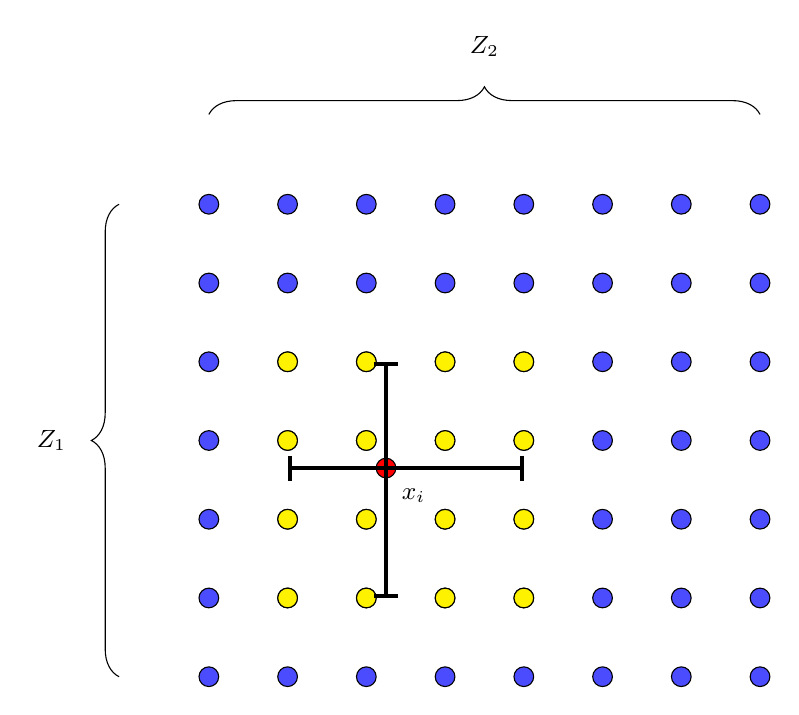
\begin{tikzpicture}
	
  \foreach \x in {1, 2, 3, 4, 5, 6, 7, 8} 
    \foreach \y in {1, 2, 3, 4, 5, 6, 7} 
      \node[circle, draw, fill=blue!70, inner sep=0pt, minimum size=0.25cm] at (\x, \y) {};

    
  \foreach \x in {2, 3, 4, 5} 
    \foreach \y in {2, 3, 4, 5} 
      \node[circle, draw, fill=yellow, inner sep=0pt, minimum size=0.25cm] at (\x, \y) {};

  \draw [decorate,decoration={brace,amplitude=10pt,raise=4pt},yshift=0pt]
    (0, 1) -- (0,7) node [black,midway,xshift=-1.cm] 
    {\small $Z_1$};

  \draw [decorate,decoration={brace,amplitude=10pt,raise=4pt},yshift=0pt]
    (1, 8) -- (8, 8) node [black,midway,yshift=1.cm] {\small $Z_2$};

  \node[circle, draw, fill=red, inner sep=0pt, minimum size=0.25cm] at (3.25, 3.65) {};
  \node[] at (3.6, 3.3) {\small $x_i$};
  \draw[|-|, line width=1.5pt] (3.25, 2) to (3.25, 5);
  \draw[|-|, line width=1.5pt] (2, 3.65) to (5, 3.65);

\end{tikzpicture}

    }
    \end{center}
    
    \begin{itemize}
      \item Inducing points can be considered as inteprolation points for the
        kernel.
        \[
          k_i \approx K_{mm} w_i,
        \]
      where $w_i\in \R^{m}$ is the vector of interpolation coefficients.

      \item KISS-GP uses cubic convolutional interpolation for which 
        \[
          w_i = w_i^1 \otimes w_i^2 \otimes \ldots \otimes w_i^D.
        \]
\end{itemize}

\section*{\LARGE \color{NavyBlue} Tensor Train Format}

\citet{oseledets2011}

Tensor $\tens{A}$ is said to be represented in TT format if:
%$$
%      \tensel{A}(i_1, \dots, i_d)
%        = \underbrace{G_1[i_1]}_{ 1 \times r} \,    
%           \underbrace{G_2[i_2]}_{ r \times r} \dotsm \underbrace{G_d[i_d]}_{ r \times 1},~~~i_k \in \{1, \ldots, n_k\}.
%$$  

%\begin{center}
%    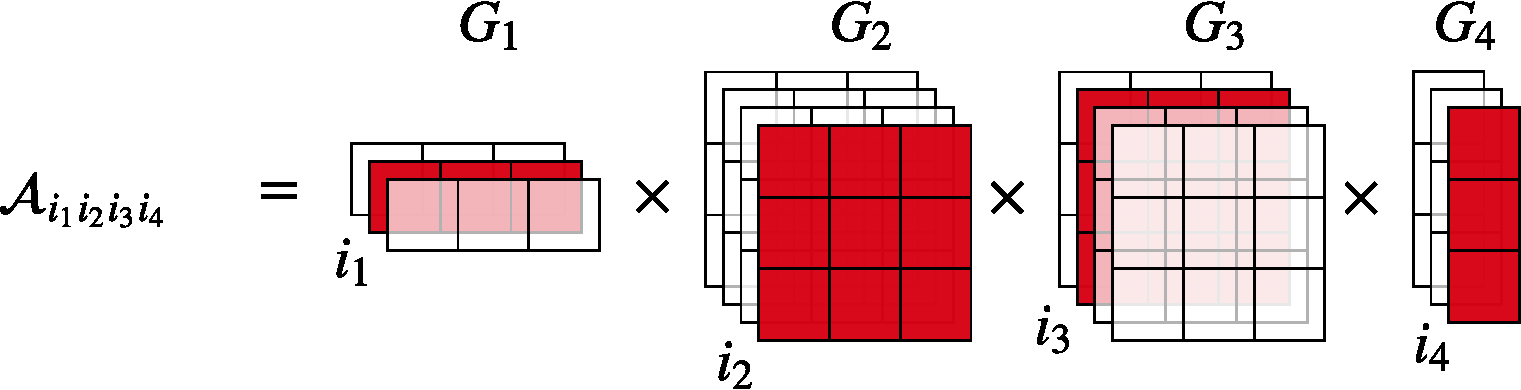
\includegraphics{pics/tt/TT_v2.pdf}
%\end{center}


%\begin{figure}
% \centering
\flushleft
\def\svgwidth{33cm}
% \renewcommand\normalsize{\tiny}%
\includesvg{pics/tt/TT}
%    \end{figure}

\begin{itemize}
  \item TT-format uses $O \left ( d n r^2 \right )$ memory to approximate a
    tensor with $n^d$ elements.
  \item Allows for efficient implementation of linear algebra operations.
\end{itemize}


\section*{\LARGE \color{NavyBlue}Gaussian Process ELBO}
    
Using KISS-GP approximation of $k_i \approx K_{mm} w_i$, we can rewrite the 
ELBO as
\[
  \log p(y) \ge \sum_{i=1}^n \bigg(\log \N (y_i | w_i^T \mu, \sigma^2) - 
  \frac 1 {2 \sigma^2} (\mbox{var}_i + w_i^T K_{mm} w_i) -\frac 1 {2 \sigma^2} 
    \tr (w_i^T \Sigma w_i)\bigg)
\]
\[
  - \frac 1 2 \bigg(\log \frac {|K_{mm}|} {|\Sigma|} - m + \tr(K_{mm}^{-1} \Sigma)
  + \mu^T K_{mm}^{-1}\mu \bigg)
\]
where
\begin{itemize}
  \item $K_{mm} \in \R^{m \times m}$ is the covariance matrix computed at the
    inducing points
  \item $k_i \in \R^m$ is the vector of covariances between the $i$-th training
    object and the inducing points
  \item $\sigma^2$ is the noise variance
  \item $\mu \in \R^m$, $\Sigma \in \R^{m \times m}$ — variational parameters
  \item $\tilde K_{ii} = \mbox{var} - k_i^T K_{mm}^{-1} k_i$, where  
    $\mbox{var}$ is the prior variance of the process at any point
\end{itemize}

\section*{\LARGE \color{NavyBlue}TT-GP}

\begin{itemize}
  \item Set inducing points $Z$ on a grid in the feature space
  \item Restrict $\Sigma$ to be in a Kronecker product format
    \[
      \Sigma = \Sigma^1 \otimes \Sigma^2\otimes \ldots \otimes \Sigma^D.
    \]
  \item Restrict $\mu$ to be in TT format with TT-ranks $r$.
\end{itemize}

\section*{\LARGE \color{NavyBlue} Properties}
    
\begin{itemize}
  \item The computational complexity is linear in the size of the data
    $\bigO(n D m^{1 / D} r^2 + D m^{1 / D} r^3 + D m^{3 / D})$. 
    TT-ranks are in general on the scale of $r \approx 10$.\\ 
    Here $m = m_0^D$.
  \item To fit the process we can use simple SGD
  \item The method can be applied for large $n$, moderately large $D$,
    and huge $m$
\end{itemize}

\section*{\LARGE \color{NavyBlue} RBF Kernel Experiments}
\citet{hensman2013}

%  \caption[]{Experimental results for standard RBF kernels. In the table acc. stands for $r^2$ for regression and accuracy
%          for classification tasks. $n$ is the size of the
%          training set, $D$ is the dimensionality of the feature space,
%          $m$ is the number of inducing inputs, $r$ is TT-ranks of $\mu$ for TT-GP; $t$ is the time per one pass over
%          the data (epoch) in seconds; where provided, $d$ is the dimensionality of linear embedding.\\
%          $^*$ for KLSP-GP on Airline we provide results from the original
%          paper where the accuracy is given as a plot, and detailed
%          information about experiment setup and exact results is not available.
%          }
%  \label{se_results}
%  \centering
\begin{center}
  \begin{tabular}{lll l cll l clll}
    \toprule
    \multicolumn{3}{c}{Dataset} && \multicolumn{3}{c}{SVI-GP / KLSP-GP} && \multicolumn{4}{c}{TT-GP} \\
    \cmidrule{1-3}
    \cmidrule{5-7}
    \cmidrule{9-12}

    Name & $n$ & $D$ &&
    acc. & $m$ & $t$ (s) &&
    acc. & $m$ & $d$ & $t$ (s)\\
    \midrule

    Powerplant & $7654$ & $4$ &&
    $0.94$ & $200$ & $10$ &&
    $0.95$ & $35^4$ & - & $5$ \\

    Protein & $36584$ & $9$ &&
    $0.50$ & $200$ & $45$ &&
    $0.56$ & $30^9$ & - & $40$ \\

    YearPred & $463K$ & $90$ &&
    $0.30$ & $1000$ & $597$ &&
    $0.32$ & $10^6$ & $6$ & $105$ \\

    \midrule
    Airline & $6M$ & $8$ &&
    $0.665^*$ & - & - &&
    $0.694$ & $20^8$ & - & $5200$ \\

    svmguide1 & 3089 & 4 &&
    $0.967$ & $200$ & $4$ &&
    $0.969$ & $20^4$ & - & $1$\\

    EEG & 11984 & 14 &&
    $0.915$ & $1000$ & $18$ &&
    $0.908$ & $12^{10}$ & $10$ & $10$\\

    covtype bin & 465K & 54 &&
    $0.817$ & $1000$ & $320$ &&
    $0.852$ & $10^6$ & $6$ & $172$\\
    \bottomrule
  \end{tabular}
\end{center}
\section*{\LARGE \color{NavyBlue} Deep Kernel Experiments}
\citet{wilson2016stochastic}
    
\begin{center}
    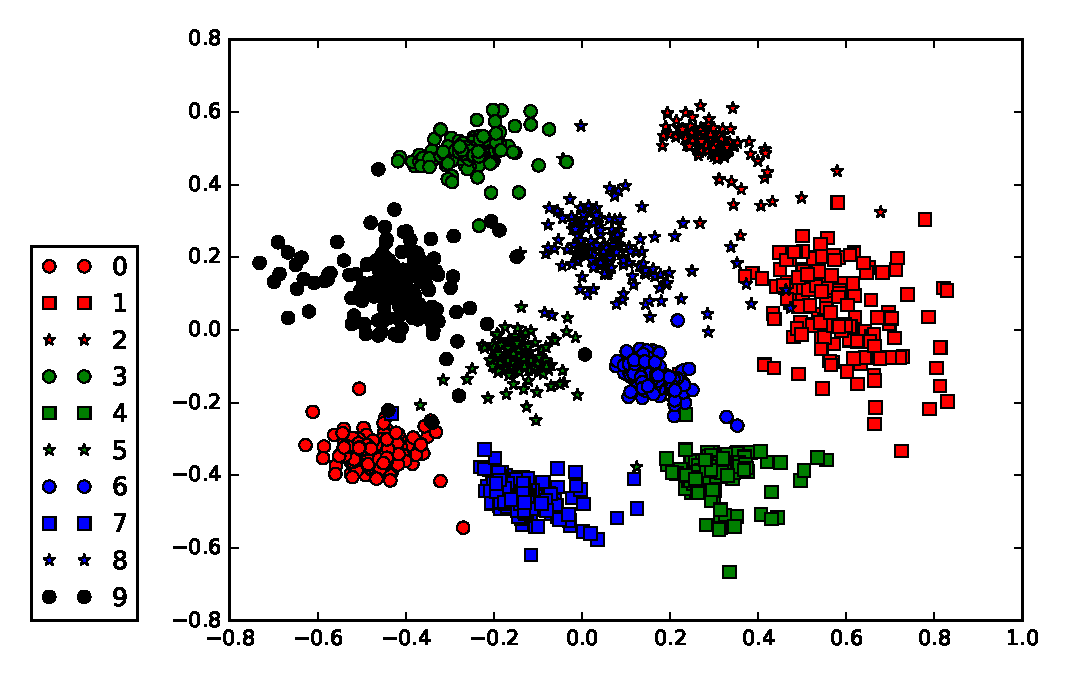
\includegraphics[width=20cm]{pics/embed/embedding_2.eps}
\end{center}

\begin{center}
%  \begin{table}[t]
%    \vspace{-.5cm}
%    \caption{Results of experiments with deep kernels. Here acc. is classification
%            accuracy; $C$ is the number of classes; $d$ is the dimensionality
%            of embedding learned by the model; $t$ is the time per one pass over
%            data (epoch) in seconds.}
    \label{deep_results}
    \centering
    \begin{tabular}{ll ll llll lll}
      \toprule
      \multicolumn{1}{c}{Dataset}  && SV-DKL &&
      \multicolumn{2}{c}{DNN} &&
      \multicolumn{3}{c}{TT-GP}\\

      \cmidrule{1-1}
      \cmidrule{3-3}
      \cmidrule{5-6}
      \cmidrule{8-10}

      Name &&
      acc. && acc. & $t$ (s) &&
      acc. & $d$ & $t$ (s)
      \\
      \midrule


      %\cmidrule{9-10}
      %\cmidrule{12-13}

      Airline && 
      $0.781$ && $0.780$ & $1055$ &&
      $0.788 \pm 0.002$ & $2$ & $1375$\\

      CIFAR-10 && 
      $-$ && $0.915$ & $166$ &&
      $0.908 \pm 0.003$ & $9$ & $220$\\

      MNIST && 
      $-$ && $0.993$ & $23$ &&
      $0.9936 \pm 0.0004$ & $10$ & $64$\\
      \bottomrule
    \end{tabular}
\end{center}


%\nocite{*} % Print all references regardless of whether they were cited in the poster or not
%\bibliographystyle{plain} % Plain referencing style
\bibliography{biblio} % Use the example bibliography file sample.bib
\bibliographystyle{plainnat}

%\section*{Acknowledgements}


\end{multicols}
\end{document}
